\documentclass{article}
\usepackage{xfrac, amssymb, amsmath, gensymb, graphicx, amsthm, mathtools}
\usepackage{semantic}
\usepackage[a4paper, total={6in, 8in}]{geometry}
\usepackage{graphicx}
\setlength{\parindent}{0pt}

\title{ECE 4740 Lab 4 Proposal}
\author{Ethan Gabizon, Nandita Nagarajan, Dylan Lee}

\begin{document}
\maketitle

\section{Implementation Plan}
We plan to implement an embedded SRAM array. We will have a 6:64 bit row decoder, so there will be 64 words in our design.
Each word will be 8 bits, so we will need a 3:8 bit column decoder. For implementing these decoders, we plan to use our lab 2
decoder. 2:4 decoders can be cascaded as follows to create a 4:16 decoder, which we will then use to implement a 6:64 decoder.

\begin{figure}[h]
    \caption{4:16 decoder using cascaded 2:4 decoders}
    \centering
    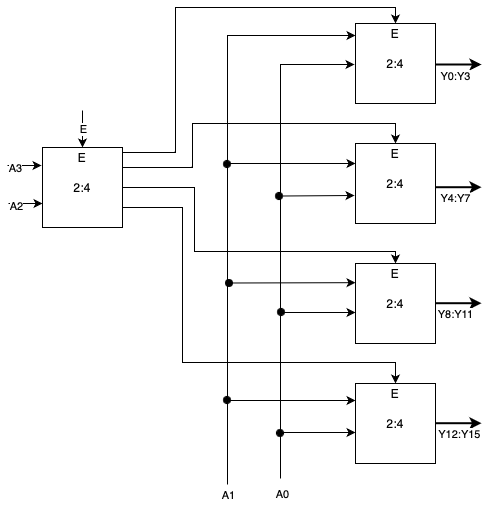
\includegraphics[width=0.3\textwidth]{4_16decoder.drawio.png}
\end{figure}

\begin{figure}[h]
    \caption{6:64 decoder using 2:4 and 4:16 decoders}
    \centering
    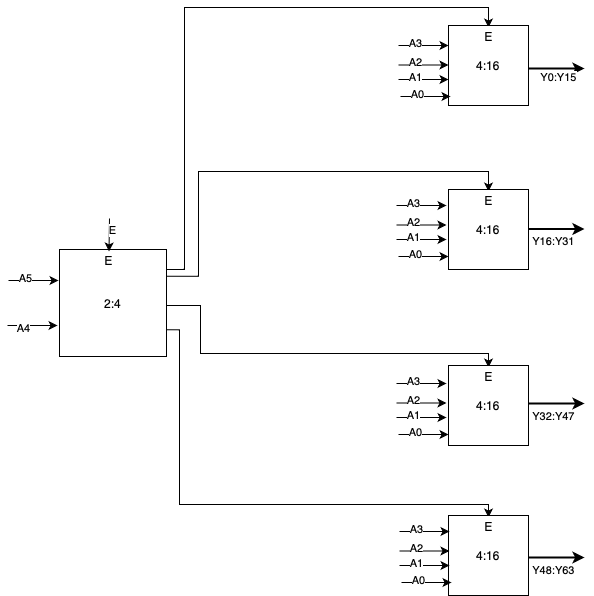
\includegraphics[width=0.3\textwidth]{6_64decoder.drawio.png}
\end{figure}

\begin{figure}[h]
    \caption{3:8 decoder using 2:4}
    \centering
    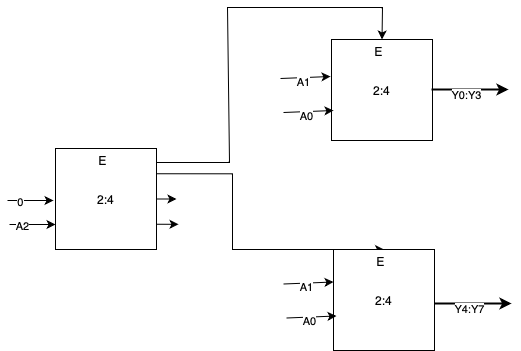
\includegraphics[width=0.3\textwidth]{3_8decoder.drawio.png}
\end{figure}

As seen in the diagrams, this will require our 2:4 decoders to have an enable signal as an input. Modifying our existing module to 
reflect this behavior is simple: we will add an AND gate at the output, where one of the inputs is the enable and the other 
is the decoder output. In total, the row and address decoder design will use 24 of our 2:4 decoders, so we can expect area to be
about 24 times the 2:4 decoder area, but possibly more since we need to add the enable signal.\newline

We will implement an SRAM cell as shown below, using 2 cross-coupled inverters.
\begin{figure}[h]
    \caption{6T SRAM cell}
    \centering
    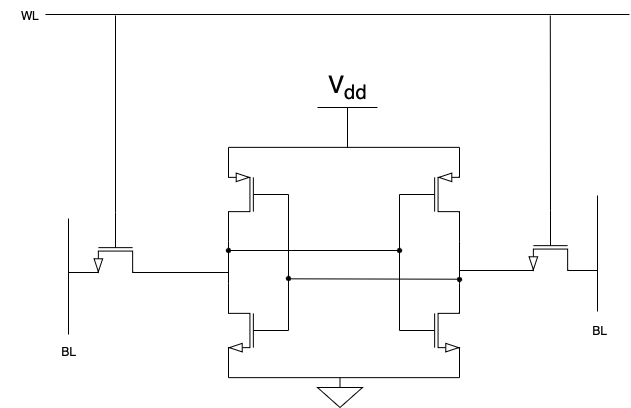
\includegraphics[width=0.3\textwidth]{sramcell.drawio.png}
\end{figure}

For our actual SRAM array, it is hard to say what the area will be. A single bit SRAM cell uses 6 transistors. Our entire SRAM array
will have a total of $64 \cdot 8 = 256$ bits, so the total area will be about 256 times the area of a single cell.

\section{Testing Plan}
We plan to incrementally test our design. This means that after implementing our 6:64 decoder, we will test it before moving on.
Our testing plan for this decoder is similar to the way we tested our lab 2 decoder. We plan to write a Matlab script that tests
each of the possible inputs of the decoder to ensure it produces the right output.\newline

With our decoder fully verified, we can then move on to testing our SRAM array. Similarly to how we tested our decoder, we plan 
to use a Matlab script that tests that each wordline is working correctly. Our script would iterate through asserting each of
the 64 wordlines, and toggling all of the bits of each word one at a time. After writing a value to each bit, we would read
from the SRAM array to ensure that the wordline is holding the correct value.

\section{Performance Evaluation}
Our goal for our evaluation is to measure the hold and read margins for one of our single SRAM cells. This will give us a 
concrete metric of how much noise our SRAM cells can handle, which is a concern with SRAM cells in the real world.

\end{document}